% Modified from pandoc --print-default-template=latex
\documentclass[oneside]{book}
\usepackage[T1]{fontenc}
\usepackage{lmodern}
\usepackage{amssymb,amsmath}
\usepackage{ifxetex,ifluatex}
\usepackage{fixltx2e} % provides \textsubscript
\usepackage{upquote}


\usepackage{mathspec}
\usepackage{xltxtra,xunicode}
\defaultfontfeatures{Mapping=tex-text,Scale=MatchLowercase}
\setmonofont[Mapping=tex-ansi]{Inconsolata}


% Taken from pandoc x.md -o test.tex --standalone
\usepackage{color}
\usepackage{fancyvrb}
\newcommand{\VerbBar}{|}
\newcommand{\VERB}{\Verb[commandchars=\\\{\}]}
\DefineVerbatimEnvironment{Highlighting}{Verbatim}{commandchars=\\\{\}}
\newenvironment{Shaded}{}{}
\newcommand{\KeywordTok} [1]{\textcolor[rgb]{0.00,0.44,0.13}{{#1}}}
\newcommand{\DataTypeTok}[1]{\textcolor[rgb]{0.56,0.13,0.00}{{#1}}}
\newcommand{\DecValTok}  [1]{\textcolor[rgb]{0.25,0.63,0.44}{{#1}}}
\newcommand{\BaseNTok}   [1]{\textcolor[rgb]{0.25,0.63,0.44}{{#1}}}
\newcommand{\FloatTok}   [1]{\textcolor[rgb]{0.25,0.63,0.44}{{#1}}}
\newcommand{\CharTok}    [1]{\textcolor[rgb]{0.25,0.44,0.63}{{#1}}}
\newcommand{\StringTok}  [1]{\textcolor[rgb]{0.25,0.44,0.63}{{#1}}}
\newcommand{\CommentTok} [1]{\textcolor[rgb]{0.38,0.63,0.69}{{#1}}}
\newcommand{\OtherTok}   [1]{\textcolor[rgb]{0.00,0.44,0.13}{{#1}}}
\newcommand{\AlertTok}   [1]{\textcolor[rgb]{1.00,0.00,0.00}{{#1}}}
\newcommand{\FunctionTok}[1]{\textcolor[rgb]{0.02,0.16,0.49}{{#1}}}
\newcommand{\ErrorTok}   [1]{\textcolor[rgb]{1.00,0.00,0.00}{{#1}}}
\newcommand{\NormalTok}  [1]{{#1}}

\usepackage{longtable}
\usepackage{booktabs}
\usepackage{graphicx}

\usepackage[hyphens]{url}
\usepackage[setpagesize=false, % page size defined by xetex
            unicode=false, % unicode breaks when used with xetex
            xetex]{hyperref}
\hypersetup{breaklinks=true,
            bookmarks=true,
            pdfauthor={},
            pdftitle={Environments},
            colorlinks=true,
            citecolor=blue,
            urlcolor=[rgb]{0.3,0.3,0.3},
            linkcolor=[rgb]{0.3,0.3,0.3},
            pdfborder={0 0 0}}

% Place links as footnotes
\renewcommand{\href}[2]{#2 (\url{#1})}
% Use ref for internal links
\renewcommand{\hyperref}[2][???]{\autoref{#1}}
\def\chapterautorefname{Chapter}
\def\sectionautorefname{Section}
\def\subsectionautorefname{Section}

\setlength{\parindent}{0pt}
\setlength{\parskip}{6pt plus 2pt minus 1pt}
\setlength{\emergencystretch}{3em}  % prevent overfull lines

\title{Environments}
\author{}
\date{}

\begin{document}



\section{Environments}\label{environments}

\subsection{Introduction}\label{introduction}

The environment is the data structure that powers scoping in R. An
environment binds names to values, and understanding how they work will
help you understand scoping more deeply. Environments are also useful
because they have reference semantics.

The binding between names and values are usually created with
\texttt{\textless{}-} or \texttt{assign()}. Other functions, like
\texttt{delayedBinding()} and \texttt{activeBinding()}, allow you to
create special bindings that work in a different way. These are rarely
useful, but are fun to learn about and play with.

\subparagraph{Outline}\label{outline}

\subparagraph{Prerequisities}\label{prerequisities}

This chapter uses many functions from the \texttt{pryr} package to pry
open R and look inside at the messy details. You can install
\texttt{pryr} by running
\texttt{devtools::install\_github("hadley/pryr")}

\subsection{Environment basics}\label{environment-basics}

The job of an environment is to associate, or \textbf{bind}, a set of
names to a set of values. You can think of an environment as a bag of
names:

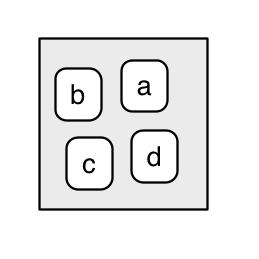
\includegraphics[width=1.18in,height=1.18in]{diagrams/environments.png/bag-of-names.png}

Each name points to an object stored elsewhere in memory:

\begin{Shaded}
\begin{Highlighting}[]
\NormalTok{e <-}\StringTok{ }\KeywordTok{new.env}\NormalTok{()}
\NormalTok{e$a <-}\StringTok{ }\OtherTok{FALSE}
\NormalTok{e$b <-}\StringTok{ "a"}
\NormalTok{e$c <-}\StringTok{ }\FloatTok{2.3}
\NormalTok{e$d <-}\StringTok{ }\DecValTok{1}\NormalTok{:}\DecValTok{3}
\end{Highlighting}
\end{Shaded}

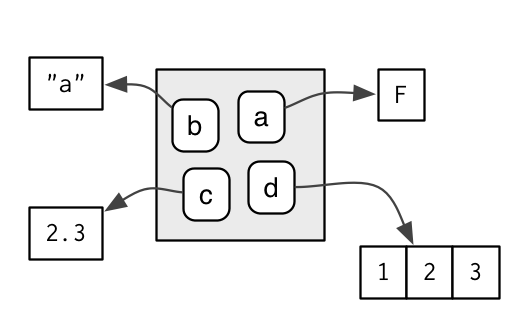
\includegraphics[width=2.36in,height=1.47in]{diagrams/environments.png/bindings.png}

The objects don't live in the environment so multiple names can point to
the same object:

\begin{Shaded}
\begin{Highlighting}[]
\NormalTok{e$a <-}\StringTok{ }\NormalTok{e$d}
\end{Highlighting}
\end{Shaded}

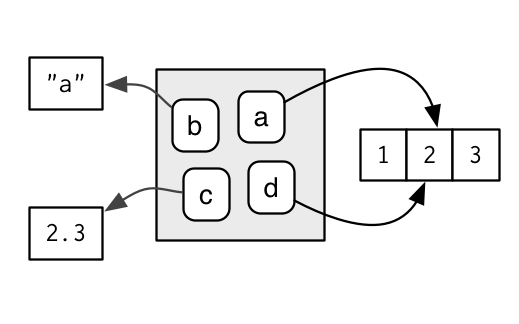
\includegraphics[width=2.36in,height=1.47in]{diagrams/environments.png/multiple-names.png}

Confusingly they can also point to different objects that have the same
value:

\begin{Shaded}
\begin{Highlighting}[]
\NormalTok{e$a <-}\StringTok{ }\DecValTok{1}\NormalTok{:}\DecValTok{3}
\end{Highlighting}
\end{Shaded}

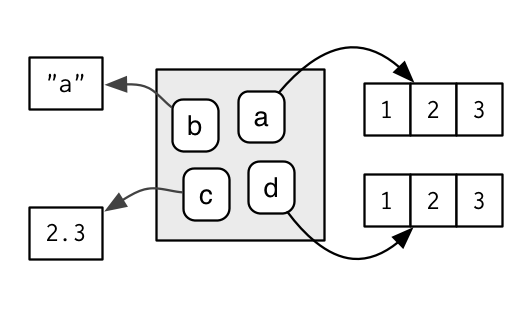
\includegraphics[width=2.36in,height=1.47in]{diagrams/environments.png/copies.png}

If an object has no names pointing to it, it gets automatically deleted
by the garbage collector. This process is described in more detail in
\hyperref[gc]{gc}.

Every environment also has a parent, another environment. In diagrams,
I'll represent the parent with a small black circle. The parent is used
to implement lexical scoping: if a name is not found in an environment,
then R will look in its parent (and so on). Only one environment doesn't
have a parent: the \textbf{empty} environment.

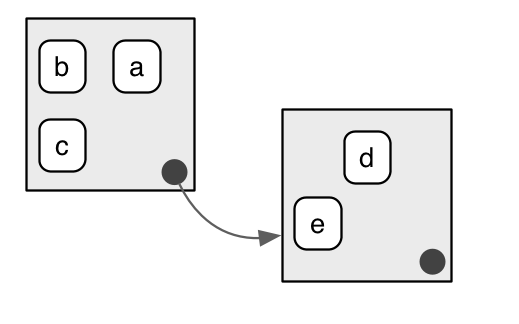
\includegraphics[width=2.36in,height=1.47in]{diagrams/environments.png/parents.png}

We use the metaphor of a family to refer to environments. The
grandparent of a environment is the parent's parent, and the ancestors
include parent environments all the way up to the empty environment.
It's rare to talk about the children of an environment because there are
no back links: given an environment we have no way to find its children.

Generally, an environment is similar to a list, with four important
exceptions:

\begin{itemize}
\item
  Every object in an environment has a unique name.
\item
  The objects in an environment are not ordered (i.e.~it doesn't make
  sense to ask what the first object in an environment is).
\item
  An environment has a parent.
\item
  Environments have reference semantics. When you modify a binding in an
  environment, the environment is not copied; it's modified in place.
  \hyperref[explicit-environments]{Explicit environments} discusses the
  implications.
\end{itemize}

More technically, an environment is made up of two components, the
\textbf{frame}, which contains the name-object bindings (and behaves
much like a named list), and the parent environment. Unfortunately
``frame'' is used inconsistently in R. For example,
\texttt{parent.frame()} doesn't give you the parent frame of an
environment, it gives you the \emph{calling} environment. This is
discussed in more details in \hyperref[calling-environments]{calling
environments}.

There are four special environments:

\begin{itemize}
\item
  \texttt{globalenv()}: the interactive workspace. This is the
  environment in which your normally work. The parent of the global
  environment is the last package that you attached with
  \texttt{library()}.
\item
  \texttt{baseenv()}: the environment of the base package. The parent of
  the base environment is the empty environment.
\item
  \texttt{emptyenv()}: the ultimate ancestor of all environments, and
  the only environment without a parent.
\item
  \texttt{environment()}: the current environment.
\end{itemize}

\texttt{search()} lists all parents of the global environment. This is
called the search path because objects in these environments can be
found from the top-level interactive workspace. It contains an
environment for each attached package and any other objects that you've
\texttt{attach()}ed. It also contains a special environment called
\texttt{Autoloads} which is used to save memory by only loading package
objects (like big datasets) when needed.

You can access the environments of any environment on the search list
using \texttt{as.environment()}.

\begin{Shaded}
\begin{Highlighting}[]
\KeywordTok{search}\NormalTok{()}
\CommentTok{#>  [1] ".GlobalEnv"        "package:bookdown"  "package:stats"    }
\CommentTok{#>  [4] "package:graphics"  "package:grDevices" "package:utils"    }
\CommentTok{#>  [7] "package:datasets"  "package:methods"   "Autoloads"        }
\CommentTok{#> [10] "package:base"}
\KeywordTok{as.environment}\NormalTok{(}\StringTok{"package:stats"}\NormalTok{)}
\CommentTok{#> <environment: package:stats>}
\CommentTok{#> attr(,"name")}
\CommentTok{#> [1] "package:stats"}
\CommentTok{#> attr(,"path")}
\CommentTok{#> [1] "/Library/Frameworks/R.framework/Versions/3.1/Resources/library/stats"}
\end{Highlighting}
\end{Shaded}

\texttt{globalenv()}, \texttt{baseenv()}, the environments on the search
path, and \texttt{emptyenv()} are connected in this diagram. Each time
you load a new package with \texttt{library()} it is inserted between
the global environment and the package that was previously at the top of
the search path.

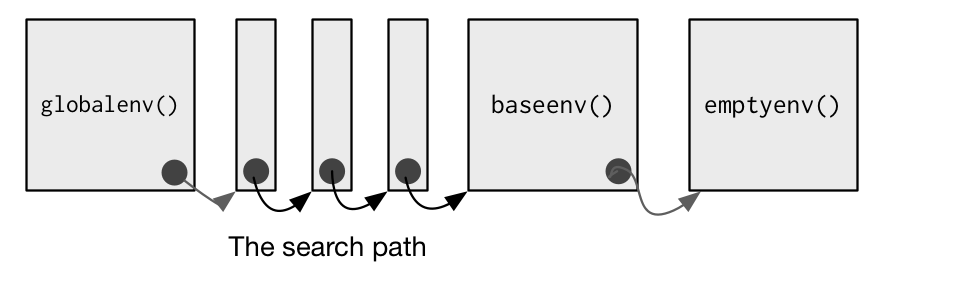
\includegraphics[width=4.43in,height=1.33in]{diagrams/environments.png/search-path.png}

To create an environment manually, use \texttt{new.env()}. You can list
the bindings in the environment's frame with \texttt{ls()} and see its
parent with \texttt{parent.env()}.

\begin{Shaded}
\begin{Highlighting}[]
\NormalTok{e <-}\StringTok{ }\KeywordTok{new.env}\NormalTok{()}
\CommentTok{# the default parent provided by new.env() is environment from }
\CommentTok{# which it is called - in this case that's the global environment.}
\KeywordTok{parent.env}\NormalTok{(e)}
\CommentTok{#> <environment: R_GlobalEnv>}
\KeywordTok{ls}\NormalTok{(e)}
\CommentTok{#> character(0)}
\end{Highlighting}
\end{Shaded}

The easiest way to modify the bindings in an environment is to treat it
like a list:

\begin{Shaded}
\begin{Highlighting}[]
\NormalTok{e$a <-}\StringTok{ }\DecValTok{1}
\NormalTok{e$b <-}\StringTok{ }\DecValTok{2}
\KeywordTok{ls}\NormalTok{(e)}
\CommentTok{#> [1] "a" "b"}
\NormalTok{e$a}
\CommentTok{#> [1] 1}
\end{Highlighting}
\end{Shaded}

By default, \texttt{ls()} only shows names that don't begin with
\texttt{.}. Use \texttt{all.names = TRUE} to show all bindings in an
environment:

\begin{Shaded}
\begin{Highlighting}[]
\NormalTok{e$.a <-}\StringTok{ }\DecValTok{2}
\KeywordTok{ls}\NormalTok{(e)}
\CommentTok{#> [1] "a" "b"}
\KeywordTok{ls}\NormalTok{(e, }\DataTypeTok{all.names =} \OtherTok{TRUE}\NormalTok{)}
\CommentTok{#> [1] ".a" "a"  "b"}
\end{Highlighting}
\end{Shaded}

Another useful way to view an environment is \texttt{ls.str()}. It is
more useful than \texttt{str()} because it shows each object in the
environment. Like \texttt{ls()}, it also has an \texttt{all.names}
argument.

\begin{Shaded}
\begin{Highlighting}[]
\KeywordTok{str}\NormalTok{(e)}
\CommentTok{#> <environment: 0x7fc13e600f50>}
\KeywordTok{ls.str}\NormalTok{(e)}
\CommentTok{#> a :  num 1}
\CommentTok{#> b :  num 2}
\end{Highlighting}
\end{Shaded}

Given a name, you can extract the value to which it is bound with
\texttt{\$}, \texttt{{[}{[}}, or \texttt{get()}:

\begin{itemize}
\item
  \texttt{\$} and \texttt{{[}{[}} look only in one environment and
  return \texttt{NULL} if there is no binding associated with the name.
\item
  \texttt{get()} uses the regular scoping rules and throws an error if
  the binding is not found.
\end{itemize}

\begin{Shaded}
\begin{Highlighting}[]
\NormalTok{e$c <-}\StringTok{ }\DecValTok{3}
\NormalTok{e$c}
\CommentTok{#> [1] 3}
\NormalTok{e[[}\StringTok{"c"}\NormalTok{]]}
\CommentTok{#> [1] 3}
\KeywordTok{get}\NormalTok{(}\StringTok{"c"}\NormalTok{, }\DataTypeTok{envir =} \NormalTok{e)}
\CommentTok{#> [1] 3}
\end{Highlighting}
\end{Shaded}

Deleting objects from environments works a little differently from
lists. With a list you can remove an entry by setting it to
\texttt{NULL}. In environments, that will create a new binding to
\texttt{NULL}. Instead, use \texttt{rm()} to remove the binding.

\begin{Shaded}
\begin{Highlighting}[]
\NormalTok{e <-}\StringTok{ }\KeywordTok{new.env}\NormalTok{()}

\NormalTok{e$a <-}\StringTok{ }\DecValTok{1}
\NormalTok{e$a <-}\StringTok{ }\OtherTok{NULL}
\KeywordTok{ls}\NormalTok{(e)}
\CommentTok{#> [1] "a"}

\KeywordTok{rm}\NormalTok{(}\StringTok{"a"}\NormalTok{, }\DataTypeTok{envir =} \NormalTok{e)}
\KeywordTok{ls}\NormalTok{(e)}
\CommentTok{#> character(0)}
\end{Highlighting}
\end{Shaded}

You can determine if a binding exists in a environment with the
\texttt{exists()} function. Like \texttt{get()}, the default is to
follow regular scoping rules and look in parent environments. If you
don't want this behavior, use \texttt{inherits = FALSE}:

\begin{Shaded}
\begin{Highlighting}[]
\NormalTok{x <-}\StringTok{ }\DecValTok{10}
\KeywordTok{exists}\NormalTok{(}\StringTok{"x"}\NormalTok{, }\DataTypeTok{envir =} \NormalTok{e)}
\CommentTok{#> [1] TRUE}
\KeywordTok{exists}\NormalTok{(}\StringTok{"x"}\NormalTok{, }\DataTypeTok{envir =} \NormalTok{e, }\DataTypeTok{inherits =} \OtherTok{FALSE}\NormalTok{)}
\CommentTok{#> [1] FALSE}
\end{Highlighting}
\end{Shaded}

To compare enviroments, you must use \texttt{identical()} not
\texttt{==}:

\begin{Shaded}
\begin{Highlighting}[]
\KeywordTok{identical}\NormalTok{(}\KeywordTok{globalenv}\NormalTok{(), }\KeywordTok{environment}\NormalTok{())}
\CommentTok{#> [1] TRUE}
\KeywordTok{globalenv}\NormalTok{() ==}\StringTok{ }\KeywordTok{environment}\NormalTok{()}
\CommentTok{#> Error: comparison (1) is possible only for atomic and list types}
\end{Highlighting}
\end{Shaded}

\subsubsection{Exercises}\label{exercises}

\begin{enumerate}
\def\labelenumi{\arabic{enumi}.}
\item
  List three ways in which an environment differs from a list.
\item
  If you don't supply an explcit environment, where do \texttt{ls()} and
  \texttt{rm()} look? Where does \texttt{\textless{}-} make bindings?
\item
  Using \texttt{parent.env()} and a loop (or a recursive function),
  verify that the ancestors of \texttt{globalenv()} include
  \texttt{baseenv()} and \texttt{emptyenv()}. Use the same basic idea to
  implement your own version of \texttt{search()}.
\end{enumerate}

\subsection{Recursing over
environments}\label{recursing-over-environments}

Environments form a tree, so it's often convenient to write a recursive
function. This section shows you how by applying your new knowledge of
environments to understand the helpful \texttt{plyr::where()}. Given a
name, \texttt{where()} that finds the environment \emph{where} it's
defined, using R's regular scoping rules:

\begin{Shaded}
\begin{Highlighting}[]
\KeywordTok{library}\NormalTok{(pryr)}
\NormalTok{x <-}\StringTok{ }\DecValTok{5}
\KeywordTok{where}\NormalTok{(}\StringTok{"x"}\NormalTok{)}
\CommentTok{#> <environment: R_GlobalEnv>}
\KeywordTok{where}\NormalTok{(}\StringTok{"mean"}\NormalTok{)}
\CommentTok{#> <environment: base>}
\end{Highlighting}
\end{Shaded}

The definition of \texttt{where()} is straightforward. It has two
arguments: the name to look for (as a string), and the environment in
which to start the search. (We'll learn later why
\texttt{parent.frame()} is a good default in
\hyperref[calling-environments]{calling environments}.)

\begin{Shaded}
\begin{Highlighting}[]
\NormalTok{where <-}\StringTok{ }\NormalTok{function(name, }\DataTypeTok{env =} \KeywordTok{parent.frame}\NormalTok{()) \{}
  \NormalTok{if (}\KeywordTok{identical}\NormalTok{(env, }\KeywordTok{emptyenv}\NormalTok{())) \{}
    \CommentTok{# Base case}
    \KeywordTok{stop}\NormalTok{(}\StringTok{"Can't find "}\NormalTok{, name, }\DataTypeTok{call. =} \OtherTok{FALSE}\NormalTok{)}
    
  \NormalTok{\} else if (}\KeywordTok{exists}\NormalTok{(name, }\DataTypeTok{envir =} \NormalTok{env, }\DataTypeTok{inherits =} \OtherTok{FALSE}\NormalTok{)) \{}
    \CommentTok{# Success case}
    \NormalTok{env}
    
  \NormalTok{\} else \{}
    \CommentTok{# Recursive case}
    \KeywordTok{where}\NormalTok{(name, }\KeywordTok{parent.env}\NormalTok{(env))}
    
  \NormalTok{\}}
\NormalTok{\}}
\end{Highlighting}
\end{Shaded}

There are three cases:

\begin{itemize}
\item
  The base case: we've reached the empty environment and haven't found
  the binding. We can't go any further, so we throw an error.
\item
  The successful case: the name exists in this environment, so we return
  the environment.
\item
  The recursive case: the name was not found in this environment, so try
  the parent.
\end{itemize}

It's easier to see what's going on with a picture. Imagine you have two
environments as in the following diagram:

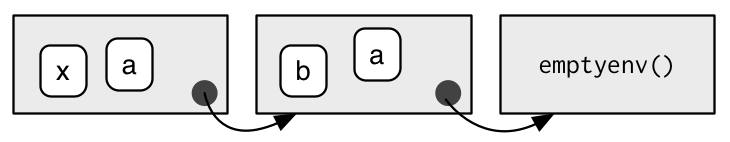
\includegraphics[width=3.32in,height=0.65in]{diagrams/environments.png/where-ex.png}

\begin{itemize}
\item
  If you're looking for \texttt{a}, \texttt{where()} will find it in the
  first environment.
\item
  If you're looking for \texttt{b}, it's not in the first environment,
  so \texttt{where()} will look in its parent and find it there.
\item
  If you're looking for \texttt{c}, it's not in the first environment,
  or the second environment, so \texttt{where()} gets to the empty
  environment and throws an error.
\end{itemize}

It's natural to work with environments recursively, so \texttt{where()}
provides a useful template to follow. Removing the specifics of
\texttt{where()} shows the structure more clearly:

\begin{Shaded}
\begin{Highlighting}[]
\NormalTok{f <-}\StringTok{ }\NormalTok{function(..., }\DataTypeTok{env =} \KeywordTok{parent.frame}\NormalTok{()) \{}
  \NormalTok{if (}\KeywordTok{identical}\NormalTok{(env, }\KeywordTok{emptyenv}\NormalTok{())) \{}
    \CommentTok{# base case}
  \NormalTok{\} else if (success) \{}
    \CommentTok{# success case}
  \NormalTok{\} else \{}
    \CommentTok{# recursive case}
    \KeywordTok{f}\NormalTok{(..., }\DataTypeTok{env =} \KeywordTok{parent.env}\NormalTok{(env))}
  \NormalTok{\}}
\NormalTok{\}}
\end{Highlighting}
\end{Shaded}

\begin{verbatim}
#> NULL
\end{verbatim}

It's possible use a loop instead of with recursion. This might run
slightly faster (because we eliminate some function calls), but I think
it's harder to understand. I include it because you might find it easier
to see what's happening if you're less familiar with recursive
functions.

\begin{Shaded}
\begin{Highlighting}[]
\NormalTok{is_empty <-}\StringTok{ }\NormalTok{function(x) }\KeywordTok{identical}\NormalTok{(x, }\KeywordTok{emptyenv}\NormalTok{())}

\NormalTok{f2 <-}\StringTok{ }\NormalTok{function(..., }\DataTypeTok{env =} \KeywordTok{parent.frame}\NormalTok{()) \{}
  \NormalTok{while(!}\KeywordTok{is_empty}\NormalTok{(env)) \{}
    \NormalTok{if (success) \{}
      \CommentTok{# success case}
      \KeywordTok{return}\NormalTok{()}
    \NormalTok{\}}
    \CommentTok{# inspect parent}
    \NormalTok{env <-}\StringTok{ }\KeywordTok{parent.env}\NormalTok{(env)}
  \NormalTok{\}}

  \CommentTok{# base case}
\NormalTok{\}}
\end{Highlighting}
\end{Shaded}

\begin{verbatim}
#> NULL
\end{verbatim}

\subsubsection{Exercises}\label{exercises-1}

\begin{enumerate}
\def\labelenumi{\arabic{enumi}.}
\item
  Modify \texttt{where()} to find all environments that contain a
  binding for \texttt{name}.
\item
  Write your own version of \texttt{get()} using a function written in
  the style of \texttt{where()}.
\item
  Write a function called \texttt{fget()} that finds only function
  objects. It should have two arguments, \texttt{name} and \texttt{env},
  and should obey the regular scoping rules for functions: if there's an
  object with a matching name that's not a function, look in the parent.
  For an added challenge, also add an \texttt{inherits} argument which
  controls whether the function recurses up the parents or only looks in
  one environment.
\item
  Write your own version of \texttt{exists(inherits = FALSE)} (Hint: use
  \texttt{ls()}). Write a recursive version that behaves like
  \texttt{exists(inherits = TRUE)}.
\end{enumerate}

\subsection{Function environments}\label{function-environments}

Most of the time, you do not create environments directly. They are
created as a consequence of working with functions. This section
discusses the four types of environments associated with a function:
enclosing, binding, execution, and calling.

The \textbf{enclosing} environment is a property of a function that is
set when it's created. Every function has one and only one enclosing
environment. For the three other types of environment, there may be 0, 1
or many environments associated with each function:

\begin{itemize}
\item
  Binding a function to a name with \texttt{\textless{}-} defines a
  \textbf{binding} environment.
\item
  Calling a function creates an ephemeral \textbf{execution} environment
  that stores variables created during execution.
\item
  Every execution environment is associated with a \textbf{calling}
  environment, which tells you where the function was called.
\end{itemize}

The following sections will explain why each of these environments are
important, how to access them, and how you might use them.

\subsubsection{The enclosing
environment}\label{the-enclosing-environment}

When a function is created, it gains a reference to the environment
where it was made. This is the \textbf{enclosing environment} and is
used for lexical scoping. When called with a function
\texttt{environment()} returns the enclosing environment:

\begin{Shaded}
\begin{Highlighting}[]
\NormalTok{y <-}\StringTok{ }\DecValTok{1}
\NormalTok{f <-}\StringTok{ }\NormalTok{function(x) x +}\StringTok{ }\NormalTok{y}
\KeywordTok{environment}\NormalTok{(f)}
\CommentTok{#> <environment: R_GlobalEnv>}
\end{Highlighting}
\end{Shaded}

In diagrams, I'll depict functions as a rounded rectangles. The
enclosing environment of a function is given by a small black circle:

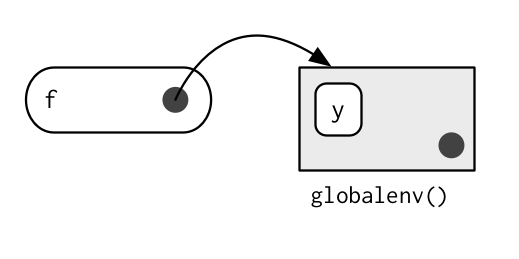
\includegraphics[width=2.06in,height=0.74in]{diagrams/environments.png/enclosing.png}

\subsubsection{Binding environments}\label{binding-environments}

The enclosing environment determines how the function finds values; the
binding environments determine how we find the function. The previous
diagram is too simple because functions don't have names. Instead, the
name of a function is defined by a binding. The binding environments of
a function are all the environments which have a binding to it. The
following diagram better reflects relatively because the the enclosing
environment contains a binding from \texttt{f} to the function:

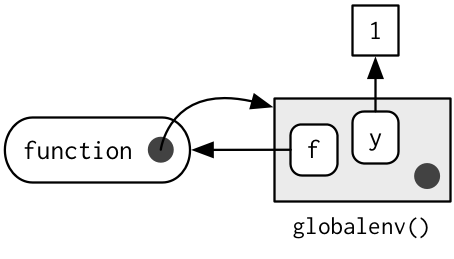
\includegraphics[width=2.06in,height=1.18in]{diagrams/environments.png/binding.png}

In this case the enclosing and binding environments are the same. They
will be differently if you assign a function into a different
environment:

\begin{Shaded}
\begin{Highlighting}[]
\NormalTok{e <-}\StringTok{ }\KeywordTok{new.env}\NormalTok{()}
\NormalTok{e$g <-}\StringTok{ }\NormalTok{function() }\DecValTok{1}
\end{Highlighting}
\end{Shaded}

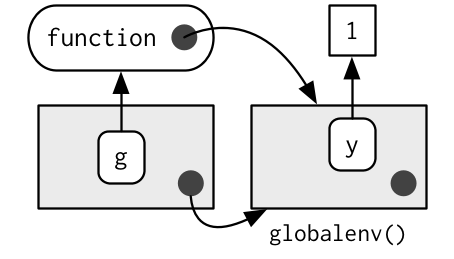
\includegraphics[width=2.06in,height=1.18in]{diagrams/environments.png/binding-2.png}

The enclosing environment belongs to the function, and never changes,
even if the function is moved to a different environment.

The distinction between the binding environment and the enclosing
environment is important because it is critical for package namespaces.
Package namespaces keep packages independent. For example, if package A
uses the base \texttt{mean()} function, what happens if package B
creates it's own \texttt{mean()} function? Namespaces ensure that
package A continues to use the base \texttt{mean()} function, and that
package A is not affected by package B (unless explicitly asked for).

Namespaces are implemented using environments, taking advantage of the
fact that functions don't have to live in their enclosing environments.
For example, take the base function \texttt{sd()}. It's binding and
enclosing environments are different:

\begin{Shaded}
\begin{Highlighting}[]
\KeywordTok{environment}\NormalTok{(sd)}
\CommentTok{#> <environment: namespace:stats>}
\KeywordTok{where}\NormalTok{(}\StringTok{"sd"}\NormalTok{)}
\CommentTok{#> <environment: package:stats>}
\CommentTok{#> attr(,"name")}
\CommentTok{#> [1] "package:stats"}
\CommentTok{#> attr(,"path")}
\CommentTok{#> [1] "/Library/Frameworks/R.framework/Versions/3.1/Resources/library/stats"}
\end{Highlighting}
\end{Shaded}

The definition of \texttt{sd()} uses \texttt{var()}, but if we make our
own version of \texttt{var()} it doesn't affect \texttt{sd()}:

\begin{Shaded}
\begin{Highlighting}[]
\NormalTok{x <-}\StringTok{ }\DecValTok{1}\NormalTok{:}\DecValTok{10}
\KeywordTok{sd}\NormalTok{(x)}
\CommentTok{#> [1] 3.028}
\NormalTok{var <-}\StringTok{ }\NormalTok{function(x, }\DataTypeTok{na.rm =} \OtherTok{TRUE}\NormalTok{) }\DecValTok{100}
\KeywordTok{sd}\NormalTok{(x)}
\CommentTok{#> [1] 3.028}
\end{Highlighting}
\end{Shaded}

This works because every package has two environments associated with
it: the \emph{package} environment and the \emph{namespace} environment.
The package environment contains every publicly accessible function, and
is place on the search path. The namespace environment contains all
functions (including internal functions), and it's parent environment is
a special imports environment that contains bindings to all the
functions that the package needs. Every exported function in a package
is bound into the \emph{package} environment, but enclosed by the
\emph{namespace} environment.

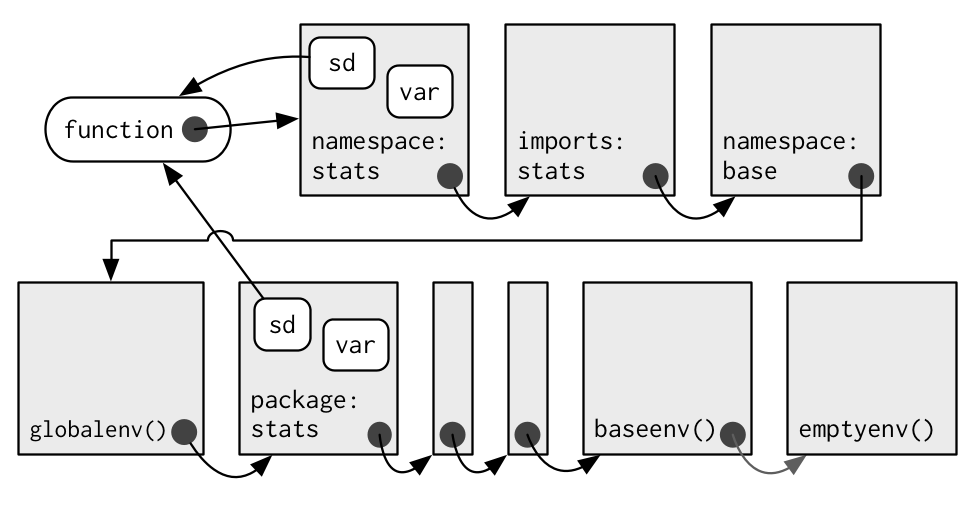
\includegraphics[width=4.43in,height=2.36in]{diagrams/environments.png/namespace.png}

When we type \texttt{var} into the console, it's found first in the
global environment. When \texttt{sd()} looks for \texttt{var()} it finds
it first in its namespace environment so never looks in the
\texttt{globalenv()}.

\subsubsection{Execution environments}\label{execution-environments}

What will the following function return the first time its run? What
about the second?

\begin{Shaded}
\begin{Highlighting}[]
\NormalTok{g <-}\StringTok{ }\NormalTok{function(x) \{}
  \NormalTok{if (!}\KeywordTok{exists}\NormalTok{(}\StringTok{"a"}\NormalTok{, }\DataTypeTok{inherits =} \OtherTok{FALSE}\NormalTok{)) \{}
    \KeywordTok{message}\NormalTok{(}\StringTok{"Defining a"}\NormalTok{)}
    \NormalTok{a <-}\StringTok{ }\DecValTok{1}
  \NormalTok{\} else \{}
    \NormalTok{a <-}\StringTok{ }\NormalTok{a +}\StringTok{ }\DecValTok{1}
  \NormalTok{\}}
  \NormalTok{a}
\NormalTok{\}}
\KeywordTok{g}\NormalTok{(}\DecValTok{10}\NormalTok{)}
\KeywordTok{g}\NormalTok{(}\DecValTok{10}\NormalTok{)}
\end{Highlighting}
\end{Shaded}

This function returns the same value every time it is called because of
the fresh start principle, described in \hyperref[a-fresh-start]{a fresh
start}. Each time a function is called, a new environment is created to
host execution. The parent of the execution environment is the enclosing
environment of the function. Once the function has completed, this
environment is thrown away.

Let's depict that graphically with a simpler function. I draw execution
environments around the function they belong to with a dotted border.

\begin{Shaded}
\begin{Highlighting}[]
\NormalTok{h <-}\StringTok{ }\NormalTok{function(x) \{}
  \NormalTok{a <-}\StringTok{ }\DecValTok{1}
  \NormalTok{x +}\StringTok{ }\NormalTok{a}
\NormalTok{\}}
\NormalTok{y <-}\StringTok{ }\KeywordTok{h}\NormalTok{(}\DecValTok{1}\NormalTok{)}
\end{Highlighting}
\end{Shaded}

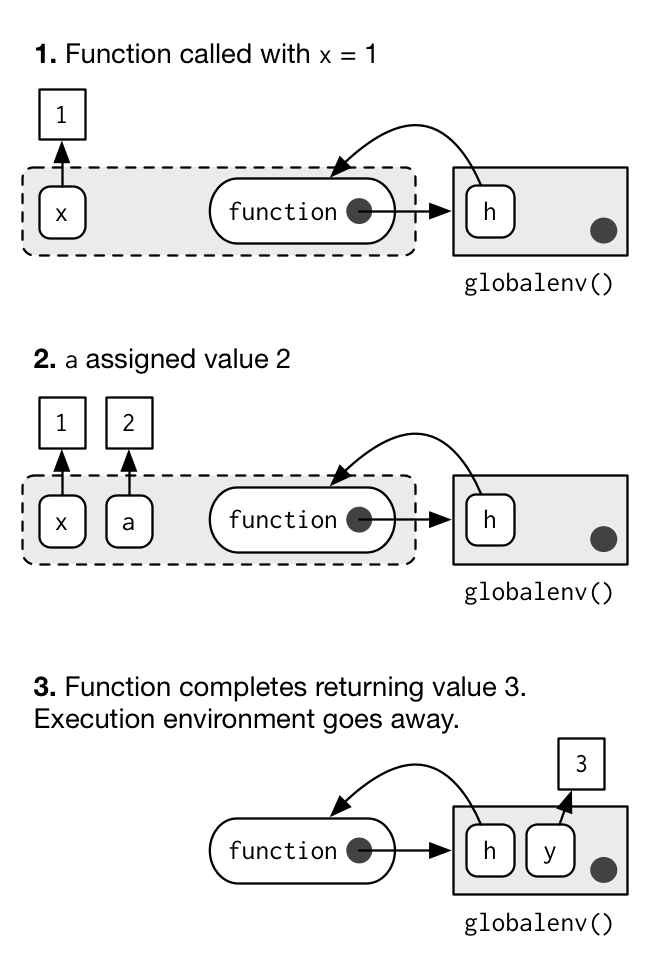
\includegraphics[width=2.95in,height=4.43in]{diagrams/environments.png/execution.png}

When you create a function inside another function, the enclosing
environment of the child is the execution environment of the parent.
When this happens, the execution environment is no longer ephemeral. The
following example illustrates that idea with a function factory,
\texttt{plus()}. We use that factory to create a function called
\texttt{plus\_one()}. The enclosing environment of \texttt{plus\_one()}
is the execution environment of \texttt{plus()} where \texttt{x} bound
to the value 1.

\begin{Shaded}
\begin{Highlighting}[]
\NormalTok{plus <-}\StringTok{ }\NormalTok{function(x) \{}
  \NormalTok{function(y) x +}\StringTok{ }\NormalTok{y}
\NormalTok{\}}
\NormalTok{plus_one <-}\StringTok{ }\KeywordTok{plus}\NormalTok{(}\DecValTok{1}\NormalTok{)}
\KeywordTok{identical}\NormalTok{(}\KeywordTok{parent.env}\NormalTok{(}\KeywordTok{environment}\NormalTok{(plus_one)), }\KeywordTok{environment}\NormalTok{(plus))}
\CommentTok{#> [1] TRUE}
\end{Highlighting}
\end{Shaded}

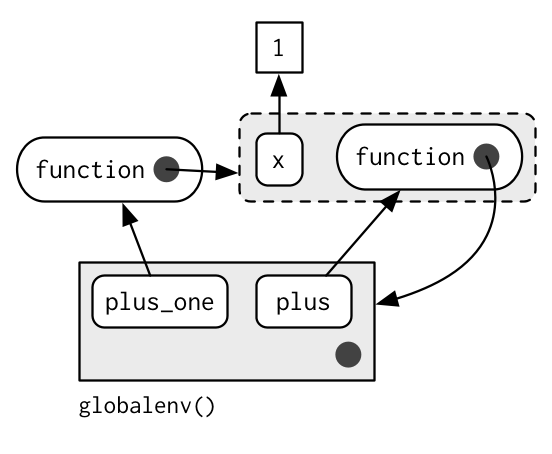
\includegraphics[width=2.51in,height=2.06in]{diagrams/environments.png/closure-2.png}

\hyperdef{}{calling-environments}{\subsubsection{Calling
environments}\label{calling-environments}}

Look at the following code. What do you expect \texttt{g()} to return
when the code is run?

\begin{Shaded}
\begin{Highlighting}[]
\NormalTok{h <-}\StringTok{ }\NormalTok{function() \{}
  \NormalTok{x <-}\StringTok{ }\DecValTok{10}
  \NormalTok{function() \{}
    \NormalTok{x}
  \NormalTok{\}}
\NormalTok{\}}
\NormalTok{i <-}\StringTok{ }\KeywordTok{h}\NormalTok{()}
\NormalTok{x <-}\StringTok{ }\DecValTok{20}
\KeywordTok{i}\NormalTok{()}
\end{Highlighting}
\end{Shaded}

The top-level \texttt{x} is a red herring: using the regular scoping
rules, \texttt{g()} looks first where it is defined and finds that the
value associated with \texttt{x} is 10. However, it's still meaningful
to ask what value \texttt{x} is associated with in the environment where
\texttt{g()} is called: \texttt{x} is 10 in the environment where
\texttt{g()} is defined, but it is 20 in the environment where
\texttt{g()} is called.

We can access this environment using the unfortunately named
\texttt{parent.frame()}. This function returns the \textbf{environment}
where the function was called. We can also use this function to look up
the value of names in that environment:

\begin{Shaded}
\begin{Highlighting}[]
\NormalTok{f2 <-}\StringTok{ }\NormalTok{function() \{}
  \NormalTok{x <-}\StringTok{ }\DecValTok{10}
  \NormalTok{function() \{}
    \NormalTok{def <-}\StringTok{ }\KeywordTok{get}\NormalTok{(}\StringTok{"x"}\NormalTok{, }\KeywordTok{environment}\NormalTok{())}
    \NormalTok{cll <-}\StringTok{ }\KeywordTok{get}\NormalTok{(}\StringTok{"x"}\NormalTok{, }\KeywordTok{parent.frame}\NormalTok{())}
    \KeywordTok{list}\NormalTok{(}\DataTypeTok{defined =} \NormalTok{def, }\DataTypeTok{called =} \NormalTok{cll)}
  \NormalTok{\}}
\NormalTok{\}}
\NormalTok{g2 <-}\StringTok{ }\KeywordTok{f2}\NormalTok{()}
\NormalTok{x <-}\StringTok{ }\DecValTok{20}
\KeywordTok{str}\NormalTok{(}\KeywordTok{g2}\NormalTok{())}
\CommentTok{#> List of 2}
\CommentTok{#>  $ defined: num 10}
\CommentTok{#>  $ called : num 20}
\end{Highlighting}
\end{Shaded}

In more complicated scenarios, there's not just one parent call, but a
sequence of calls which lead all the way back to the initiating
function, called from the top-level. The following code generates a call
stack three levels deep. The open-ended arrows represent the caling
environment of each execution environment.

\begin{Shaded}
\begin{Highlighting}[]
\NormalTok{x <-}\StringTok{ }\DecValTok{0}
\NormalTok{y <-}\StringTok{ }\DecValTok{10}
\NormalTok{f <-}\StringTok{ }\NormalTok{function() \{}
  \NormalTok{x <-}\StringTok{ }\DecValTok{1}
  \KeywordTok{g}\NormalTok{()}
\NormalTok{\}}
\NormalTok{g <-}\StringTok{ }\NormalTok{function() \{}
  \NormalTok{x <-}\StringTok{ }\DecValTok{2}
  \KeywordTok{h}\NormalTok{()}
\NormalTok{\}}
\NormalTok{h <-}\StringTok{ }\NormalTok{function() \{}
  \NormalTok{x <-}\StringTok{ }\DecValTok{3}
  \NormalTok{x +}\StringTok{ }\NormalTok{y}
\NormalTok{\}}
\KeywordTok{f}\NormalTok{()}
\CommentTok{#> [1] 13}
\end{Highlighting}
\end{Shaded}

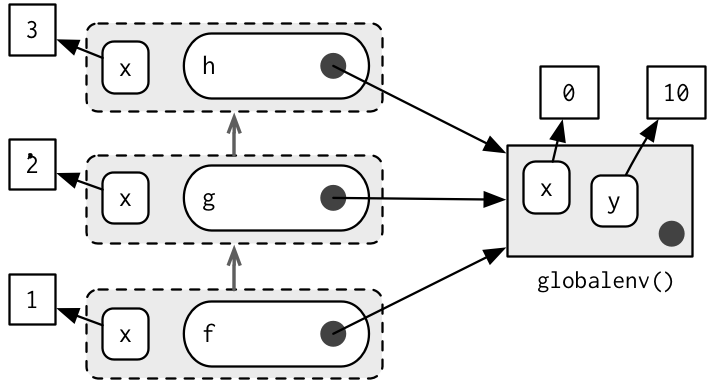
\includegraphics[width=3.25in,height=1.77in]{diagrams/environments.png/calling.png}

Note that each execution environment has two parents: a calling
environment and an enclosing environment. R's regular scoping rules only
use the enclosing parent; \texttt{parent.frame()} allows you to access
the calling parent.

Looking up variables in the calling environment rather than in the
enclosing environment is called \textbf{dynamic scoping}. Few languages
implement dynamic scoping (Emacs Lisp is a
\href{http://www.gnu.org/software/emacs/emacs-paper.html\#SEC15}{notable
exception}). This is because dynamic scoping makes it much harder to
reason about how a function operates: not only do you need to know how
it was defined, you also need to know in what context it was called.
Dynamic scoping is primarily useful for developing functions that aid
interactive data analysis. It is one of the topics discussed in
\hyperref[nse]{non-standard evaluation}.

\subsubsection{Exercises}\label{exercises-2}

\begin{enumerate}
\def\labelenumi{\arabic{enumi}.}
\item
  List the four environments associated with a function. What does each
  one do? Why is the distinction between enclosing and binding
  environments particularly important?
\item
  Draw a diagram that shows the enclosing environments of this function:

\begin{Shaded}
\begin{Highlighting}[]
\NormalTok{f1 <-}\StringTok{ }\NormalTok{function(x1) \{}
  \NormalTok{f2 <-}\StringTok{ }\NormalTok{function(x2) \{}
    \NormalTok{f3 <-}\StringTok{ }\NormalTok{function(x3) \{}
      \NormalTok{x1 +}\StringTok{ }\NormalTok{x2 +}\StringTok{ }\NormalTok{x3}
    \NormalTok{\}}
    \KeywordTok{f3}\NormalTok{(}\DecValTok{3}\NormalTok{)}
  \NormalTok{\}}
  \KeywordTok{f2}\NormalTok{(}\DecValTok{2}\NormalTok{)}
\NormalTok{\}}
\KeywordTok{f1}\NormalTok{(}\DecValTok{1}\NormalTok{)}
\end{Highlighting}
\end{Shaded}
\item
  Expand your previous diagram to show function bindings.
\item
  Expand it again to show the execution and calling environments.
\item
  Write an enhanced version of \texttt{str()} that provides more
  information about functions. Show where the function was found and
  what environment it was defined in.
\end{enumerate}

\hyperdef{}{explicit-environments}{\subsection{Explicit
environments}\label{explicit-environments}}

As well as powering scoping, environments are also useful data
structures in their own right because they have \textbf{reference
semantics}. Unlike most objects in R, when you modify an environment, it
does not make a copy. For example, look at this \texttt{modify()}
function.

\begin{Shaded}
\begin{Highlighting}[]
\NormalTok{modify <-}\StringTok{ }\NormalTok{function(x) \{}
  \NormalTok{x$a <-}\StringTok{ }\DecValTok{2}
  \KeywordTok{invisible}\NormalTok{()}
\NormalTok{\}}
\end{Highlighting}
\end{Shaded}

If you apply it to a list, the original list is not changed because
modifying a list actually modifies a copy.

\begin{Shaded}
\begin{Highlighting}[]
\NormalTok{x_l <-}\StringTok{ }\KeywordTok{list}\NormalTok{()}
\NormalTok{x_l$a <-}\StringTok{ }\DecValTok{1}
\KeywordTok{modify}\NormalTok{(x_l)}
\NormalTok{x_l$a}
\CommentTok{#> [1] 1}
\end{Highlighting}
\end{Shaded}

However, if you apply it to an environment, the original environment
\emph{is} modified:

\begin{Shaded}
\begin{Highlighting}[]
\NormalTok{x_e <-}\StringTok{ }\KeywordTok{new.env}\NormalTok{()}
\NormalTok{x_e$a <-}\StringTok{ }\DecValTok{1}
\KeywordTok{modify}\NormalTok{(x_e)}
\NormalTok{x_e$a}
\CommentTok{#> [1] 2}
\end{Highlighting}
\end{Shaded}

This behaviour is often called reference semantics, because you can
think of every binding to an environment as a reference to the same
environment.

Just as you can use a list to pass data between functions, you can also
use an environment. When creating your own environment, note that you
should set its environment to the empty environment. This ensures you
don't accidentally inherit objects from somewhere else:

\begin{Shaded}
\begin{Highlighting}[]
\NormalTok{x <-}\StringTok{ }\DecValTok{1}
\NormalTok{e1 <-}\StringTok{ }\KeywordTok{new.env}\NormalTok{()}
\KeywordTok{get}\NormalTok{(}\StringTok{"x"}\NormalTok{, e1)}
\CommentTok{#> [1] 1}

\NormalTok{e2 <-}\StringTok{ }\KeywordTok{new.env}\NormalTok{(}\DataTypeTok{parent =} \KeywordTok{emptyenv}\NormalTok{())}
\KeywordTok{get}\NormalTok{(}\StringTok{"x"}\NormalTok{, e2)}
\CommentTok{#> Error: object 'x' not found}
\end{Highlighting}
\end{Shaded}

Environments are useful data structures for solve three common problems:

\begin{itemize}
\itemsep1pt\parskip0pt\parsep0pt
\item
  Avoiding copies of large data.
\item
  Managing state within a package.
\item
  Efficiently lookup values from names
\end{itemize}

These are described in turn below.

\subsubsection{Avoiding copies}\label{avoiding-copies}

Since environments have reference semantics, you'll never accidentally
create a copy. This makes it a useful vessel for large objects. It's a
common technique for bioconductor packages which often have to manage
large genomic objects. Changes to R 3.1.0 have made this use
substantially less important because modifying a list no longer makes a
deep copy. Previously, modifying a single element of a list would cause
every element to be copied, an expensive operation if some elements are
large. Now, modifying a list efficiently reuses existing vectors, saving
much time.

\subsubsection{Package state}\label{package-state}

Explicit environments are useful in packages because they allow you to
maintain state across function calls. A typical use case looks like
this:

\begin{Shaded}
\begin{Highlighting}[]
\NormalTok{my_env <-}\StringTok{ }\KeywordTok{new.env}\NormalTok{(}\DataTypeTok{parent =} \KeywordTok{emptyenv}\NormalTok{())}
\NormalTok{my_env$a <-}\StringTok{ }\DecValTok{1}

\NormalTok{get_a <-}\StringTok{ }\NormalTok{function() \{}
  \NormalTok{my_env$a}
\NormalTok{\}}
\NormalTok{set_a <-}\StringTok{ }\NormalTok{function(value) \{}
  \NormalTok{old <-}\StringTok{ }\NormalTok{my_env$a}
  \NormalTok{my_env$a <-}\StringTok{ }\NormalTok{value}
  \KeywordTok{invisible}\NormalTok{(old)}
\NormalTok{\}}
\end{Highlighting}
\end{Shaded}

Returning the old value from setter functions is a good pattern because
it makes it easier to reset the previous value in conjunction with
\texttt{on.exit()} (See more in \hyperref[on-exit]{on exit}. )

\subsubsection{As a hashmap}\label{as-a-hashmap}

A hashmap is a data structure that takes constant, O(1), time to find an
object based on its name. Environments provide this behaviour by
default, so can be used to simulate a hashmap. See the CRAN package
\texttt{hash} for a complete development of this idea.

\subsection{Explicit scoping with
\texttt{local}}\label{explicit-scoping-with-local}

Sometimes it's useful to be able to create a new scope without embedding
inside a function. The \texttt{local()} function allows you to do
exactly that. For example, to make an operation easier to understand,
you can make temporary variables. In this example, \texttt{df()} is
created in the global environment, but \texttt{x} and \texttt{y} are
not:

\begin{Shaded}
\begin{Highlighting}[]
\NormalTok{df <-}\StringTok{ }\KeywordTok{local}\NormalTok{(\{}
  \NormalTok{x <-}\StringTok{ }\DecValTok{1}\NormalTok{:}\DecValTok{10}
  \NormalTok{y <-}\StringTok{ }\KeywordTok{runif}\NormalTok{(}\DecValTok{10}\NormalTok{)}
  \KeywordTok{data.frame}\NormalTok{(}\DataTypeTok{x =} \NormalTok{x, }\DataTypeTok{y =} \NormalTok{y)}
\NormalTok{\})}
\end{Highlighting}
\end{Shaded}

This is equivalent to:

\begin{Shaded}
\begin{Highlighting}[]
\NormalTok{df <-}\StringTok{ }\NormalTok{(function() \{}
  \NormalTok{x <-}\StringTok{ }\DecValTok{1}\NormalTok{:}\DecValTok{10}
  \NormalTok{y <-}\StringTok{ }\KeywordTok{runif}\NormalTok{(}\DecValTok{10}\NormalTok{)}
  \KeywordTok{data.frame}\NormalTok{(}\DataTypeTok{x =} \NormalTok{x, }\DataTypeTok{y =} \NormalTok{y)}
\NormalTok{\})()}
\end{Highlighting}
\end{Shaded}

(If you're familiar with JavaScript you've probably seen this pattern
before. It's the immediately invoked function expression (IIFE). It's
used extensively by many JavaScript libraries to avoid polluting the
global namespace.)

\subsection{Assignment: binding names to values}\label{binding}

Assignment is the act of binding (or rebinding) a name to a value in an
environment. It is the counterpart to scoping, the set of rules that
determines how to find the value associated with a name. Compared to
most languages, R has extremely flexible tools for binding names to
values. In fact, you can not only bind values to names, but you can also
bind expressions (promises) or even functions, so that every time you
access the value associated with a name, you get something different!

The remainder of this section will discuss the four main ways of binding
names to values in R:

\begin{itemize}
\item
  With the regular behaviour, \texttt{name \textless{}- value}, the name
  is immediately associated with the value in the current environment.
  \texttt{assign("name", value)} works similarly, but allows assignment
  in any environment.
\item
  The double arrow, \texttt{name \textless{}\textless{}- value}, assigns
  in a similar way to variable lookup, so that
  \texttt{i \textless{}\textless{}- i + 1} modifies the binding of the
  original \texttt{i}, which is not necessarily in the current
  environment.
\item
  Lazy assignment, \texttt{delayedAssign("name", expression)}, binds an
  expression that isn't evaluated until you look up the name.
\item
  Active assignment,
  \texttt{makeActiveBinding("name", function, environment)} binds the
  name to a function, so it is ``active'' and can return a different
  value each time the name is found.
\end{itemize}

\subsubsection{Regular binding}\label{regular-binding}

You have probably used regular assignment in R thousands of times.
Regular assignment immediately creates a binding between a name and a
value in the current environment.

There are two types of names: syntactic and non-syntactic. Generally,
syntactic names consist of letters, digits, \texttt{.} and \texttt{\_},
and must start with a letter or \texttt{.} not followed by a number (so
\texttt{.a} and \texttt{.\_} are syntactic but \texttt{.1} is not).
There are also a number of reserved words (e.g. \texttt{TRUE},
\texttt{NULL}, \texttt{if}, \texttt{function}, see
\texttt{make.names()}). A syntactic name can be used on the left hand
side of \texttt{\textless{}-}:

\begin{Shaded}
\begin{Highlighting}[]
\NormalTok{a <-}\StringTok{ }\DecValTok{1}
\NormalTok{._ <-}\StringTok{ }\DecValTok{2}
\NormalTok{a_b <-}\StringTok{ }\DecValTok{3}
\end{Highlighting}
\end{Shaded}

A name can be any sequence of characters, but if it's non-syntactic you
need to do a little more work and surround the name in backticks:

\begin{Shaded}
\begin{Highlighting}[]
\StringTok{`}\DataTypeTok{a + b}\StringTok{`} \NormalTok{<-}\StringTok{ }\DecValTok{3}
\StringTok{`}\DataTypeTok{:)}\StringTok{`} \NormalTok{<-}\StringTok{ "smile"}
\StringTok{`}\DataTypeTok{    }\StringTok{`} \NormalTok{<-}\StringTok{ "spaces"}
\KeywordTok{ls}\NormalTok{()}
\CommentTok{#  [1] "    "   ":)"     "a + b"}
\StringTok{`}\DataTypeTok{:)}\StringTok{`}
\CommentTok{#  [1] "smile"}
\end{Highlighting}
\end{Shaded}

You can also create non-syntactic bindings using single and double
quotes instead of backticks, but I don't recommend it. The ability to
use strings on the left hand side of the assignment error is a
historical artefact, needed before R supported backticks.

\texttt{\textless{}-} creates a binding in the current environment.
There are three techniques to create a binding in another environment:

\begin{itemize}
\item
  Treat the environment like a list.

\begin{Shaded}
\begin{Highlighting}[]
\NormalTok{e <-}\StringTok{ }\KeywordTok{new.env}\NormalTok{()}
\NormalTok{e$a <-}\StringTok{ }\DecValTok{1}
\end{Highlighting}
\end{Shaded}
\item
  Use \texttt{assign()}, which has three important arguments: the name,
  the value, and the environment in which to create the binding.

\begin{Shaded}
\begin{Highlighting}[]
\NormalTok{e <-}\StringTok{ }\KeywordTok{new.env}\NormalTok{()}
\KeywordTok{assign}\NormalTok{(}\StringTok{"a"}\NormalTok{, }\DecValTok{1}\NormalTok{, }\DataTypeTok{envir =} \NormalTok{e)}
\end{Highlighting}
\end{Shaded}
\item
  Evaluate \texttt{\textless{}-} inside the environment. (More on this
  in \hyperref[nse]{evaluation}.)

\begin{Shaded}
\begin{Highlighting}[]
\NormalTok{e <-}\StringTok{ }\KeywordTok{new.env}\NormalTok{()}

\KeywordTok{eval}\NormalTok{(}\KeywordTok{quote}\NormalTok{(a <-}\StringTok{ }\DecValTok{1}\NormalTok{), e)}
\CommentTok{# alternatively, you can use the helper function evalq}
\CommentTok{# evalq(x, e) is exactly equivalent to eval(quote(x), e)}
\KeywordTok{evalq}\NormalTok{(a <-}\StringTok{ }\DecValTok{1}\NormalTok{, e)}
\end{Highlighting}
\end{Shaded}
\end{itemize}

I generally prefer to use the first form because it is so compact.
However, you'll see all three forms in R code in the wild.

\paragraph{Constants}\label{constants}

There's one extension to regular binding: constants. Constats are names
whose values can not be changed; they can only be bound once, and never
re-bound. We can simulate constants in R using \texttt{lockBinding()},
or the infix \texttt{\%\textless{}c-\%} found in pryr:

\begin{Shaded}
\begin{Highlighting}[]
\NormalTok{x <-}\StringTok{ }\DecValTok{10}
\KeywordTok{lockBinding}\NormalTok{(}\StringTok{"x"}\NormalTok{, }\KeywordTok{globalenv}\NormalTok{())}
\NormalTok{x <-}\StringTok{ }\DecValTok{15}
\CommentTok{#> Error: cannot change value of locked binding for 'x'}
\KeywordTok{rm}\NormalTok{(x)}

\NormalTok{x %<c-%}\StringTok{ }\DecValTok{20}
\NormalTok{x <-}\StringTok{ }\DecValTok{30}
\CommentTok{#> Error: cannot change value of locked binding for 'x'}
\KeywordTok{rm}\NormalTok{(x)}
\end{Highlighting}
\end{Shaded}

\texttt{lockBinding()} is used to prevent you from modifying objects
inside packages:

\begin{Shaded}
\begin{Highlighting}[]
\KeywordTok{assign}\NormalTok{(}\StringTok{"mean"}\NormalTok{, function(x) }\KeywordTok{sum}\NormalTok{(x) /}\StringTok{ }\KeywordTok{length}\NormalTok{(x), }\DataTypeTok{env =} \KeywordTok{baseenv}\NormalTok{())}
\CommentTok{#> Error: cannot change value of locked binding for 'mean'}
\end{Highlighting}
\end{Shaded}

\subsubsection{\texttt{\textless{}\textless{}-}}\label{section}

Another way to modify the binding between a name and its value is
\texttt{\textless{}\textless{}-}. The regular assignment arrow,
\texttt{\textless{}-}, always creates a variable in the current
environment. The special assignment arrow,
\texttt{\textless{}\textless{}-}, never creates a variable in the
current environment, but instead modifies an existing variable found by
walking up the parent environments.

\begin{Shaded}
\begin{Highlighting}[]
\NormalTok{x <-}\StringTok{ }\DecValTok{0}
\NormalTok{f <-}\StringTok{ }\NormalTok{function() \{}
  \NormalTok{g <-}\StringTok{ }\NormalTok{function() \{}
    \NormalTok{x <<-}\StringTok{ }\DecValTok{2}
  \NormalTok{\}}
  \NormalTok{x <-}\StringTok{ }\DecValTok{1}
  \KeywordTok{g}\NormalTok{()}
  \NormalTok{x}
\NormalTok{\}}
\KeywordTok{f}\NormalTok{()}
\CommentTok{#> [1] 2}
\NormalTok{x}
\CommentTok{#> [1] 0}

\NormalTok{h <-}\StringTok{ }\NormalTok{function() \{}
  \NormalTok{x <-}\StringTok{ }\DecValTok{1}
  \NormalTok{x <<-}\StringTok{ }\DecValTok{2}
  \NormalTok{x}
\NormalTok{\}}
\KeywordTok{h}\NormalTok{()}
\CommentTok{#> [1] 1}
\NormalTok{x}
\CommentTok{#> [1] 2}
\end{Highlighting}
\end{Shaded}

If \texttt{\textless{}\textless{}-} doesn't find an existing variable,
it will create one in the global environment. This is usually
undesirable, because global variables introduce non-obvious dependencies
between functions.

\texttt{name \textless{}\textless{}- value} is equivalent to
\texttt{assign("name", value, inherits = TRUE)}.

To give you more idea how this works, we could implement
\texttt{\textless{}\textless{}-} ourselves. I'm going to call it
\texttt{rebind()}, and emphasise that it's normally used to modify an
existing binding. We'll implement it with our recursive recipe for
working with environments. For the base case, we'll throw an error
(where \texttt{\textless{}\textless{}-} would assign in the global
environment), which emphasises that this should only be used to modify
existing bindings. Otherwise, we check to see if the name is found in
the current environment: if it is, we do the assignment there; if not,
we recurse.

\begin{Shaded}
\begin{Highlighting}[]
\NormalTok{rebind <-}\StringTok{ }\NormalTok{function(name, value, }\DataTypeTok{env =} \KeywordTok{parent.frame}\NormalTok{()) \{}
  \NormalTok{if (}\KeywordTok{identical}\NormalTok{(env, }\KeywordTok{emptyenv}\NormalTok{())) \{}
    \KeywordTok{stop}\NormalTok{(}\StringTok{"Can't find "}\NormalTok{, name, }\DataTypeTok{call. =} \OtherTok{FALSE}\NormalTok{)}
  \NormalTok{\} else if (}\KeywordTok{exists}\NormalTok{(name, }\DataTypeTok{envir =} \NormalTok{env, }\DataTypeTok{inherits =} \OtherTok{FALSE}\NormalTok{)) \{}
    \KeywordTok{assign}\NormalTok{(name, value, }\DataTypeTok{envir =} \NormalTok{env)}
  \NormalTok{\} else \{}
    \KeywordTok{rebind}\NormalTok{(name, value, }\KeywordTok{parent.env}\NormalTok{(env))}
  \NormalTok{\}}
\NormalTok{\}}
\KeywordTok{rebind}\NormalTok{(}\StringTok{"a"}\NormalTok{, }\DecValTok{10}\NormalTok{)}
\NormalTok{a <-}\StringTok{ }\DecValTok{5}
\KeywordTok{rebind}\NormalTok{(}\StringTok{"a"}\NormalTok{, }\DecValTok{10}\NormalTok{)}
\NormalTok{a}
\CommentTok{#> [1] 10}

\NormalTok{f <-}\StringTok{ }\NormalTok{function() \{}
  \NormalTok{g <-}\StringTok{ }\NormalTok{function() \{}
    \KeywordTok{rebind}\NormalTok{(}\StringTok{"x"}\NormalTok{, }\DecValTok{2}\NormalTok{)}
  \NormalTok{\}}
  \NormalTok{x <-}\StringTok{ }\DecValTok{1}
  \KeywordTok{g}\NormalTok{()}
  \NormalTok{x}
\NormalTok{\}}
\KeywordTok{f}\NormalTok{()}
\CommentTok{#> [1] 2}
\end{Highlighting}
\end{Shaded}

\hyperref[closures]{Closures} shows why you might want to use
\texttt{\textless{}\textless{}-} in practice.

\subsubsection{Delayed bindings}\label{delayed-bindings}

Another special type of assignment is a delayed binding: rather than
assigning the result of an expression immediately, it creates and stores
a promise to evaluate the expression when needed (much like the default
lazy evaluation of arguments in R functions). We can create delayed
bindings with the special assignment operator
\texttt{\%\textless{}d-\%}, provided by the pryr package.

\begin{Shaded}
\begin{Highlighting}[]
\KeywordTok{library}\NormalTok{(pryr)}
\KeywordTok{system.time}\NormalTok{(b %<d-%}\StringTok{ }\NormalTok{\{}\KeywordTok{Sys.sleep}\NormalTok{(}\DecValTok{1}\NormalTok{); }\DecValTok{1}\NormalTok{\})}
\CommentTok{#>    user  system elapsed }
\CommentTok{#>       0       0       0}
\KeywordTok{system.time}\NormalTok{(b)}
\CommentTok{#>    user  system elapsed }
\CommentTok{#>       0       0       1}
\end{Highlighting}
\end{Shaded}

Note that we need to be careful with more complicated expressions
because user-created infix functions have very high precedence. They're
higher in precedence than every other infix operator apart from
\texttt{\^{}}, \texttt{\$}, \texttt{@}, and \texttt{::}. For example,
\texttt{x \%\textless{}d-\% a + b} is interpreted as
\texttt{(x \%\textless{}d-\% a) + b}, so we need to use parentheses
ourselves:

\begin{Shaded}
\begin{Highlighting}[]
\NormalTok{x %<d-%}\StringTok{ }\NormalTok{(a +}\StringTok{ }\NormalTok{b)}
\NormalTok{a <-}\StringTok{ }\DecValTok{5}
\NormalTok{b <-}\StringTok{ }\DecValTok{5}
\NormalTok{x}
\CommentTok{#> [1] 10}
\end{Highlighting}
\end{Shaded}

\texttt{\%\textless{}d-\%} is a wrapper around the base
\texttt{delayedAssign()} function, which you may need to use directly if
you need more control. \texttt{delayedAssign()} has four parameters:

\begin{itemize}
\itemsep1pt\parskip0pt\parsep0pt
\item
  \texttt{x}: a variable name given as a quoted string
\item
  \texttt{value}: an unquoted expression to be assigned to x
\item
  \texttt{eval.env}: the environment in which to evaluate the expression
\item
  \texttt{assign.env}: the environment in which to create the binding
\end{itemize}

Writing \texttt{\%\textless{}d-\%} is straightforward, bearing in mind
that \texttt{makeActiveBinding} uses non-standard evaluation to capture
the representation of the second argument, so we need to use substitute
to construct the call manually. Once you've read
\hyperref[nse]{non-standard evaluation}, you might want to read the
source code and think about how it works.

One application of \texttt{delayedAssign} is \texttt{autoload}, a
function that powers \texttt{library()}. \texttt{autoload} makes R
behave as if the code and data in a package is loaded in memory, but it
doesn't actually do any work until you call one of the functions or
access a dataset. This is the way that data sets in most packages work -
you can call (e.g.) \texttt{diamonds} after \texttt{library(ggplot2)}
and it just works, but it isn't loaded into memory unless you actually
use it.

\subsubsection{Active bindings}\label{active-bindings}

You can create \textbf{active} bindings where the value is recomputed
every time you access the name:

\begin{Shaded}
\begin{Highlighting}[]
\NormalTok{x %<a-%}\StringTok{ }\KeywordTok{runif}\NormalTok{(}\DecValTok{1}\NormalTok{)}
\NormalTok{x}
\CommentTok{#> [1] 0.1797}
\NormalTok{x}
\CommentTok{#> [1] 0.8897}
\end{Highlighting}
\end{Shaded}

\texttt{\%\textless{}a-\%} is a wrapper for the base function
\texttt{makeActiveBinding()}. You may want to use this function directly
if you want more control. It has three arguments:

\begin{itemize}
\item
  \texttt{sym}: a variable name, represented as a name object or a
  string.
\item
  \texttt{fun}: a single argument function. Getting the value of
  \texttt{sym} calls \texttt{fun} with zero arguments, and setting the
  value of \texttt{sym} calls \texttt{fun} with one argument, the value.
\item
  \texttt{env}: the environment in which to create the binding.
\end{itemize}

\subsubsection{Exercises}\label{exercises-3}

\begin{enumerate}
\def\labelenumi{\arabic{enumi}.}
\item
  In \texttt{rebind()} it's unlikely that we want to assign in an
  ancestor of the global environment (i.e.~a loaded package), so modify
  the function to avoid recursing past the global environment.
\item
  Create a version of \texttt{assign()} that will only bind new names,
  never re-bind old names. Some programming languages only do this, and
  are known as
  \href{http://en.wikipedia.org/wiki/Assignment_(computer_science)\#Single_assignment}{single
  assignment} languages.
\item
  Implement \texttt{str()} for environments. Your function should list
  all bindings in the environment, and briefly describe their contents
  (you might want to use \texttt{str()} recursively). Indicate if
  bindings are active (\texttt{bindingIsActive()}) or locked
  (\texttt{bindingIsLocked()}).
\item
  Write an assignment function that can do active, delayed and locked
  bindings. What might you call it? What arguments should it take? Can
  you guess which sort of assignment it should do based on the input?
\end{enumerate}



\end{document}
